%%
%% kit-prog-tutorial
%%
%% Slides for my Java programming tutorial at KIT using LaTeX beamer.
%%
%% Copyright (c) 2015-2016 YouniS Bensalah <younis.bensalah@gmail.com>
%%
%% This work is released to the public domain.
%% For the full copyright and license information, please view the LICENSE file.
%%

\documentclass[18pt]{beamer}

\usepackage{templates/beamerthemekit}

\usepackage[utf8]{inputenc}
\usepackage{hyperref}
\usepackage{listings}

\titleimage{road}

\newcommand{\tagline}{The Type, the Variable and the Operator}
\newcommand{\quotes}[1]{``#1''}

\title[Programmieren\hspace{2.5pt}--\hspace{2.5pt}\tagline]{\tagline}
\subtitle{Programmieren~\textbar~Tutorium 32}

\author{YouniS Bensalah}
\date{7. November 2016}

\institute{Chair for Software Design and Quality}

\usepackage[citestyle=authoryear,bibstyle=numeric,hyperref,backend=biber]{biblatex}
\addbibresource{templates/example.bib}
\bibhang1em

\begin{document}

% remove annoying figure prefix in caption
\setbeamertemplate{caption}{\raggedright\insertcaption\par}

\selectlanguage{english}

\begin{frame}
    \titlepage
\end{frame}

% \begin{frame}{Heute}
%     \tableofcontents
% \end{frame}

\section{Datentypen}

\begin{frame}{Datentypen}
    \begin{block}{Datentyp}
        Ein Datentyp bezeichnet eine \textbf{Menge \quotes{gleichartiger} Elemente}.
    \end{block}
\end{frame}

\begin{frame}{Datentypen in Java}
    \begin{itemize}
        \item In Java gibt es 8 \textbf{primitive} Datentypen
        \pause
        \item Jede \textbf{Klasse} ist auch ein Datentyp
    \end{itemize}
\end{frame}

\begin{frame}{Primitive Datentypen in Java}
    \center
    \begin{tabular}{l | l | r}
        \textbf{Datentyp} & \textbf{Beschreibung} & \textbf{Beispiel} \\
        \hline
        \texttt{boolean} & Wahrheitswerte & \texttt{true}, \texttt{false} \\
        \hline
        \texttt{byte} & 8-bit Ganzzahlen & \texttt{42}, \texttt{-23} \\
        \texttt{short} & 16-bit Ganzzahlen & \texttt{42}, \texttt{-23} \\
        \texttt{int} & 32-bit Ganzzahlen & \texttt{42}, \texttt{-23} \\
        \texttt{long} & 64-bit Ganzzahlen & \texttt{42L}, \texttt{-23l} \\
        \hline
        \texttt{float} & 32-bit Gleitkommazahlen (IEEE 754) & \texttt{9.81F}, \texttt{1.602e-19f} \\
        \texttt{double} & 64-bit Gleitkommazahlen (IEEE 754) & \texttt{9.81}, \texttt{1.602E-19} \\
        \hline
        \texttt{char} & 16-bit (Unicode-)Zeichen & \texttt{'J'}, \texttt{'\textbackslash u03BB'} \\
    \end{tabular}
\end{frame}

\begin{frame}{Klasse als Datentyp: \texttt{String}}
    \begin{itemize}
        \item Die Klasse \texttt{String} repräsentiert eine \textbf{Zeichenkette}
        \begin{itemize}
            \item \texttt{String a = "Hallo";}
        \end{itemize}
        \pause
        \item Konkatenation durch \texttt{+}
        \begin{itemize}
            \item \texttt{a + " Welt"}
        \end{itemize}
        \pause
        \item \texttt{String} ist eine Klasse!
    \end{itemize}
\end{frame}


\section{Variablen}

\begin{frame}{Variablen}
    \begin{block}{Variable}
        Eine Variable ist ein \textbf{Bezeichner für eine \quotes{Stelle im Speicher}}.
    \end{block}
\end{frame}

\begin{frame}{Deklaration und Zuweisung}
    \begin{itemize}
        \item Deklaration: \textit{Typ Variablenname;}
        \begin{itemize}
            \item \texttt{int answer;}
            \item \texttt{String name;}
        \end{itemize}
        \pause
        \item Zuweisung: \textit{Variablenname = Ausdruck;}
        \begin{itemize}
            \item \texttt{answer = 42;}
            \item \texttt{name = "Jem";}
            \item \texttt{total = quantity * price;}
        \end{itemize}
        \pause
        \item Deklaration + Zuweisung: \textit{Typ Variablenname = Ausdruck;}
        \begin{itemize}
            \item \texttt{int answer = 42;}
            \item \texttt{String name = "Jem";}
        \end{itemize}
        \pause
        \vspace{.1in}
        \item \textbf{Tipp:} Immer sofort bei Deklaration auch einen Wert zuweisen.
    \end{itemize}
\end{frame}

\begin{frame}{Variable vs. Attribut}
    \textbf{Variablen}
    \pause
    \begin{itemize}
        \item Lokal
        \item Sichtbar innerhalb einer Methode
        \item Zwischenergebnis
    \end{itemize}
    \pause
    \textbf{Attribute}
    \pause
    \begin{itemize}
        \item Eigenschaft einer Klasse
        \item Sichtbar in \textit{allen} Methoden
        \item Teil der Modellierung
    \end{itemize}
\end{frame}


\section{Operatoren}

\begin{frame}{Operatoren}
    In Java gibt es:
    \begin{itemize}
        \item Arithmetische Operatoren
        \item Boolesche Operatoren
        \item Operatoren für Vergleiche
        \item Operatoren zur Manipulation von Bits
        \item Zuweisungsoperatoren
        \item \dots
    \end{itemize}
\end{frame}

\begin{frame}{Arithmetische Operatoren}
    \center
    \begin{tabular}{l | l | l}
        \textbf{Operator} & \textbf{Beschreibung} & \textbf{Beispiel} \\
        \hline
        \texttt{+} & Addition & \texttt{40 + 2} \\
        \texttt{-} & Subtraktion & \texttt{48 - 6} \\
        \texttt{*} & Multiplikation & \texttt{2 * 21} \\
        \texttt{/} & Division & \texttt{84 / 2} \\
        \texttt{\%} & Modulo (Rest) & \texttt{99 \% 57} \\
        \hline
        \texttt{-} & negatives Vorzeichen & \texttt{-x} \\
        \texttt{++} & Preinkrement bzw. Postinkrement & \texttt{++i}, \texttt{i++} \\
        \texttt{--} & Predekrement bzw. Postdekrement & \texttt{--i}, \texttt{i--} \\
    \end{tabular}
\end{frame}

\begin{frame}{Boolesche Operatoren}
    \center
    \begin{tabular}{l | l | l}
        \textbf{Operator} & \textbf{Beschreibung} & \textbf{Beispiel} \\
        \hline
        \texttt{!} & Negation & \texttt{!bad} \\
        \texttt{\&\&} & Und & \texttt{weatherIsGood = sunny \&\& dry} \\
        \texttt{||} & Oder & \texttt{needBreak = hungry || thirsty} \\
        \texttt{\textasciicircum} & exklusives Oder (XOR) & \texttt{yummy = salty \textasciicircum ~sweet} \\
    \end{tabular}
\end{frame}

\begin{frame}{Operatoren für Vergleiche}
    \center
    \begin{tabular}{l | l | l}
        \textbf{Operator} & \textbf{Beschreibung} & \textbf{Beispiel} \\
        \hline
        \texttt{==} & gleich & \texttt{4 == 4} \\
        \texttt{!=} & ungleich & \texttt{4 != 3} \\
        \texttt{>} & größer als & \texttt{4 > 3} \\
        \texttt{<} & kleiner als & \texttt{-4 < -3} \\
        \texttt{>=} & größer als oder gleich & \texttt{4 >= 4} \\
        \texttt{<=} & kleiner als oder gleich & \texttt{3 <= 3} \\
    \end{tabular}
\end{frame}

\begin{frame}{Operatoren zur Manipulation von Bits}
    \center
    \begin{tabular}{l | l | l}
        \textbf{Operator} & \textbf{Beschreibung} & \textbf{Beispiel} \\
        \hline
        \texttt{\textasciitilde} & invertiert alle Bits & \texttt{\textasciitilde x} \\
        \texttt{\&} & bitweises Und & \texttt{7 \& 5} \\
        \texttt{|} & bitweises Oder & \texttt{7 | 5} \\
        \texttt{\textasciicircum} & bitweises XOR & \texttt{8 \textasciicircum ~5} \\
        \hline
        \texttt{<<} & left shift & \texttt{4 << 2} \\
        \texttt{>>} & arithmetic right shift & \texttt{-2 >> 1} \\
        \texttt{>>>} & logical right shift & \texttt{-2 >>> 1} \\
    \end{tabular}
\end{frame}

\begin{frame}{Zuweisungsoperatoren}
    \center
    \begin{tabular}{l | l | l}
        \textbf{Operator} & \textbf{Beschreibung} & \textbf{Beispiel} \\
        \hline
        \texttt{=} & einfache Zuweisung & \texttt{seven = 42;} \\
        \texttt{+=} & Addition und Zuweisung & \texttt{seven += 4;} \\
        \texttt{-=} & Subtraktion und Zuweisung & \texttt{seven -= 6;} \\
        \texttt{*=} & Multiplikation und Zuweisung & \texttt{seven *= 2;} \\
        \texttt{/=} & Division und Zuweisung & \texttt{seven /= 4;} \\
        \texttt{\%=} & Modulo und Zuweisung & \texttt{seven \%= 13;} \\
    \end{tabular}
\end{frame}

\section{Quiz}

\begin{frame}[fragile]{Quiz: Was kommt raus?}
    \begin{lstlisting}[language=Java]
boolean a = true;
boolean b = false;
    \end{lstlisting}
    \begin{exampleblock}{}
        \begin{lstlisting}[language=Java]
a && b || a
        \end{lstlisting}
    \end{exampleblock}
\end{frame}

\begin{frame}[fragile]{Quiz: Was kommt raus?}
    \begin{lstlisting}[language=Java]
boolean a = true;
boolean b = false;
    \end{lstlisting}
    \begin{block}{}
        \begin{lstlisting}[language=Java]
true
        \end{lstlisting}
    \end{block}
\end{frame}

\begin{frame}[fragile]{Quiz: Was kommt raus?}
    \begin{lstlisting}[language=Java]
boolean a = true;
boolean b = false;
    \end{lstlisting}
    \begin{exampleblock}{}
        \begin{lstlisting}[language=Java]
(!a && b) || (a && !b)
        \end{lstlisting}
    \end{exampleblock}
\end{frame}

\begin{frame}[fragile]{Quiz: Was kommt raus?}
    \begin{lstlisting}[language=Java]
boolean a = true;
boolean b = false;
    \end{lstlisting}
    \begin{block}{}
        \begin{lstlisting}[language=Java]
true
        \end{lstlisting}
    \end{block}
\end{frame}

\begin{frame}[fragile]{Quiz: Was kommt raus?}
    \begin{lstlisting}[language=Java]
boolean a = true;
boolean b = false;
    \end{lstlisting}
    \begin{exampleblock}{}
        \begin{lstlisting}[language=Java]
!(!(a && b) ^ !(a || b))
        \end{lstlisting}
    \end{exampleblock}
\end{frame}

\begin{frame}[fragile]{Quiz: Was kommt raus?}
    \begin{lstlisting}[language=Java]
boolean a = true;
boolean b = false;
    \end{lstlisting}
    \begin{block}{}
        \begin{lstlisting}[language=Java]
false
        \end{lstlisting}
    \end{block}
\end{frame}

\begin{frame}[fragile]{Quiz: Was kommt raus?}
    \begin{exampleblock}{}
        \begin{lstlisting}[language=Java]
(123456 / 100) % 10
        \end{lstlisting}
    \end{exampleblock}
\end{frame}

\begin{frame}[fragile]{Quiz: Was kommt raus?}
    \begin{block}{}
        \begin{lstlisting}[language=Java]
4
        \end{lstlisting}
    \end{block}
\end{frame}

\begin{frame}[fragile]{Quiz: Was kommt raus?}
    \begin{exampleblock}{}
        \begin{lstlisting}[language=Java]
(123456 / 1000) % 10
        \end{lstlisting}
    \end{exampleblock}
\end{frame}

\begin{frame}[fragile]{Quiz: Was kommt raus?}
    \begin{block}{}
        \begin{lstlisting}[language=Java]
3
        \end{lstlisting}
    \end{block}
\end{frame}

\begin{frame}[fragile]{Quiz: Was kommt raus?}
    \begin{exampleblock}{}
        \begin{lstlisting}[language=Java]
(123456 / 10000) % 10
        \end{lstlisting}
    \end{exampleblock}
\end{frame}

\begin{frame}[fragile]{Quiz: Was kommt raus?}
    \begin{block}{}
        \begin{lstlisting}[language=Java]
2
        \end{lstlisting}
    \end{block}
\end{frame}

\begin{frame}[fragile]{Quiz: Was kommt raus?}
    \begin{exampleblock}{}
        \begin{lstlisting}[language=Java]
(2048 >> 4) % 86
        \end{lstlisting}
    \end{exampleblock}
\end{frame}

\begin{frame}[fragile]{Quiz: Was kommt raus?}
    \begin{block}{}
        \begin{lstlisting}[language=Java]
42
        \end{lstlisting}
    \end{block}
\end{frame}


\begin{frame}[fragile]{Quiz: Was kommt raus?}
    \begin{exampleblock}{}
        \begin{lstlisting}[language=Java]
3 ^ 2
        \end{lstlisting}
    \end{exampleblock}
\end{frame}

\begin{frame}[fragile]{Quiz: Was kommt raus?}
    \begin{block}{}
        \begin{lstlisting}[language=Java]
1
        \end{lstlisting}
    \end{block}
\end{frame}

\appendix

\beginbackup

\begin{frame}{Bonus Track: Enum}
    \begin{block}{Enum}
        Ein \textbf{Aufzählungstyp} (\textit{enumerated type}) ist ein Datentyp für Variablen mit einer endlichen Wertemenge.
    \end{block}
\end{frame}

\begin{frame}{Enum}
    \begin{exampleblock}{Was ist alles ein Enum?}
        \begin{itemize}
            \item Wochentage
            \item Monate
            \item Himmelsrichtungen
            \item Grundfarben (RGB)
            \item Zustände eines endlichen Automaten
            \item \dots
        \end{itemize}
    \end{exampleblock}
\end{frame}

\begin{frame}[fragile]{Enum in Java}
    \begin{lstlisting}[language=Java]
enum Day {
    MONDAY,
    TUESDAY,
    WEDNESDAY,
    THURSDAY,
    FRIDAY,
    SATURDAY,
    SUNDAY
}
    \end{lstlisting}
\end{frame}

\begin{frame}{Tipp 14: Use enums.}
    \begin{itemize}
        \item \texttt{if (today == Day.FRIDAY)} ist lesbarer als \texttt{if (today == 5)}
        \item Es schleichen sich nicht so leicht Fehler ein
        \begin{itemize}
            \item Ist \quotes{Montag} oder \quotes{Sonntag} der erste Tag der Woche?
            \item Fängt man hier bei 0 oder bei 1 an zu zählen?
            \item Welche Werte sind nochmal gültig?
            \item Ich bin Mathematiker und mag keine Zahlen
        \end{itemize}
    \end{itemize}
\end{frame}

\begin{frame}{Read the fine manual}
    \begin{itemize}
        \item \textbf{Primitive Data Types}
        \begin{itemize}
            \item \url{https://docs.oracle.com/javase/tutorial/java/nutsandbolts/datatypes.html}
        \end{itemize}
        \item \textbf{Variables}
        \begin{itemize}
            \item \url{https://docs.oracle.com/javase/tutorial/java/nutsandbolts/variables.html}
        \end{itemize}
        \item \textbf{Operators}
        \begin{itemize}
            \item \url{https://docs.oracle.com/javase/tutorial/java/nutsandbolts/operators.html}
        \end{itemize}
        \item \textbf{Enum}
        \begin{itemize}
            \item \url{https://docs.oracle.com/javase/tutorial/java/javaOO/enum.html}
        \end{itemize}
    \end{itemize}
\end{frame}

\begin{frame}{Fragen?}
    \begin{figure}
        
\includegraphics[scale=.3]{img/fragen.jpg}
    \end{figure}
\end{frame}

\begin{frame}{Bis nächste Woche!}
    \begin{figure}
        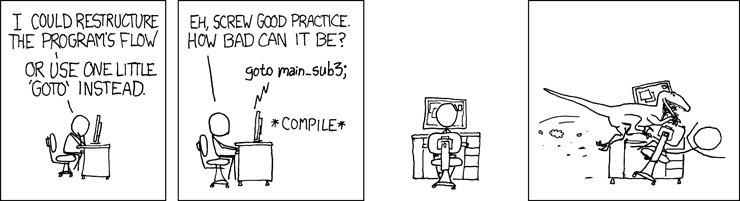
\includegraphics[scale=4]{img/goto.png}
        \caption{\footnotesize{xkcd.com}}
    \end{figure}
\end{frame}

\backupend

\end{document}
